% convex-ramp-noneq.tex

\section{Hypersonic, nonequilibrium flow over a convex ramp.}
\label{sec:convex-ramp-noneq}
%
This is a variation on the convex-ramp hypersonic flow studied by Mohammadian\,\cite{mohammadian_1972a}
in the Imperial College gun tunnel, bringing in a thermal-nonequilibrium model for the air.
We use the same static free-stream conditions as in Sec.\,\ref{sec:cubic-ramp}
but now assume that the vibrational temperature of the molecules is frozen 
at a temperature not far below the stagnation temperature.
The hope is that the extra vibrational energy will be lead to an extra bit of heat flux at the ramp surface.

\bigskip
\subsection{Input script (.py)}
%
The user input script now needs to specify the gas model as a mixture of N2 and O2 molecules and
their vibrational temperatures, when specifying the flow conditions.
Also, it needs to specify the thermal nonequilibrium energy exchange scheme (\verb!N2-O2-TV.lua!).

\noindent
\topbar
\lstinputlisting[language={}]{../2D/convex-ramp/thermo-noneq/convex-ramp.py}
\bottombar

\noindent
\topbar
\lstinputlisting[language={}]{../2D/convex-ramp/thermo-noneq/N2-O2-TV.lua}
\bottombar


\bigskip
\subsection{Running the simulation}
%
In terms of required computer time, 
this simulation is significantly more demanding than the ideal-air simulation,
taking more than 30 hours on a 4-core workstation (up from 12 hours).
The job scipts are essentially the same as for the ideal-air case.

\subsection{Results}
%
Figure\,\ref{fig:convex-ramp-noneq-field-data} shows some of the flow field data 
at $t$=1\,ms after flow start.
This is sufficient time for the flow to reach steady state.

\begin{figure}[htbp]
 \centering
 \subfloat[Pressure field.]{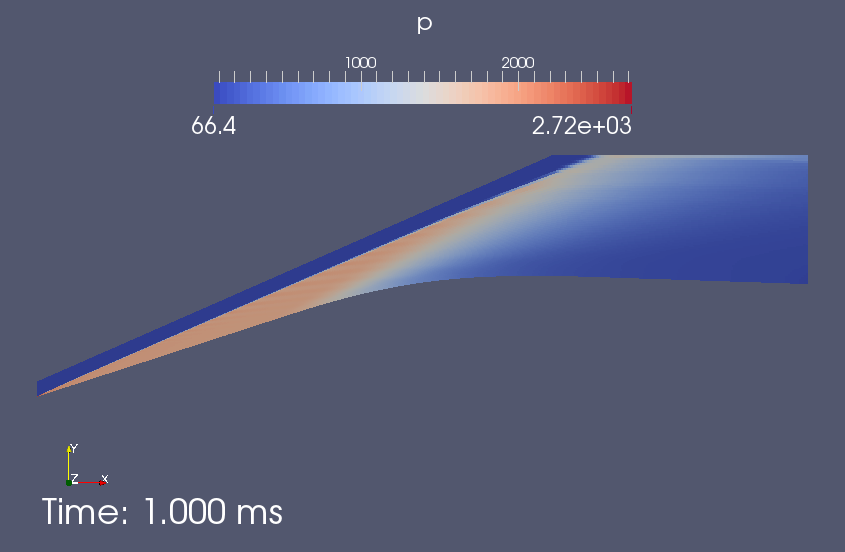
\includegraphics[width=0.65\textwidth]
    {../2D/convex-ramp/thermo-noneq/convex-ramp-factor-2-p-field-1ms.png}\label{fig:convex-ramp-noneq-pressure}}\\
 \subfloat[Static temperature field.]{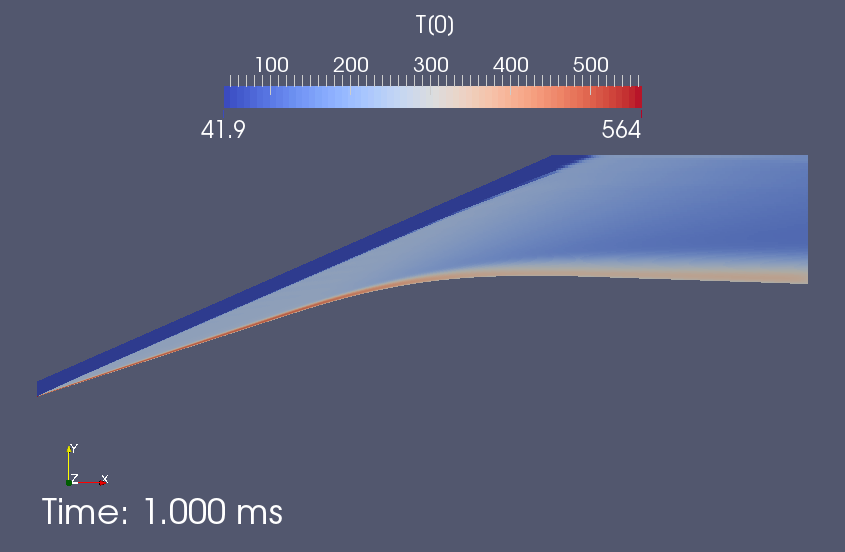
\includegraphics[width=0.65\textwidth]
    {../2D/convex-ramp/thermo-noneq/convex-ramp-factor-2-T0-field-1ms.png}\label{fig:convex-ramp-noneq-static-temperature}}\\
 \subfloat[Vibrational temperature field.]{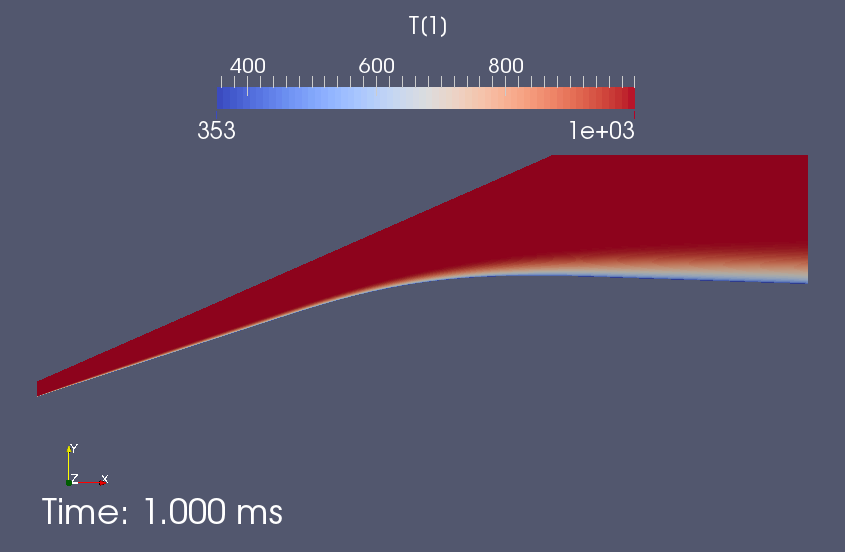
\includegraphics[width=0.65\textwidth]
    {../2D/convex-ramp/thermo-noneq/convex-ramp-factor-2-T1-field-1ms.png}\label{fig:convex-ramp-noneq-vib-temperature}}
 \caption{Computed flow field at $t$=1\,ms.}
 \label{fig:convex-ramp-noneq-field-data}
\end{figure}

\medskip
Again, the pressure field shows a nice, straight shock propagating into the free-stream, 
with an almost constant pressure region between the shock and the straight ramp surface.
The static temperature field, again, shows clearly the boundary layer that grows along the ramp surface.
The first vibrational temperature shows a relaxation toward the static temperature as the gas approaches 
the ramp surface.


\medskip
Although the computed flow field looks plausible, again,
the real proof of success of the simulation is in comparison with the experimental data.
Figure\,\ref{fig:convex-ramp-noneq-data-compare} shows the pressure and heat-transfer
along the surface of the ramp.
The simulation has done essentially the same good job of estimating the pressure distribution over the full ramp,
with a mismatch in magnitude only after passing over the faired section to reach the 
very low pressure conditions.
This pressure distribution is indistinguishable from the distribution for the ideal air simulation.
The simulation has again done a reasonable job on the heat transfer estimate,
with a small improvement over that computed in the ideal air simulation.
That agreement is good in form but only fair in magnitude is now emphasised by scaling the Eilmer3 result
by 1.2 and seeing that it falls very nicely onto the experimental data.
What is the correct answer remains unclear since the original Cheng and modified Cheng theories, 
as used by Mohammadian fall closer to the unscaled Eilmer3 result.  Sigh...

\begin{figure}[htbp]
 \centering
 \subfloat[Pressure.]{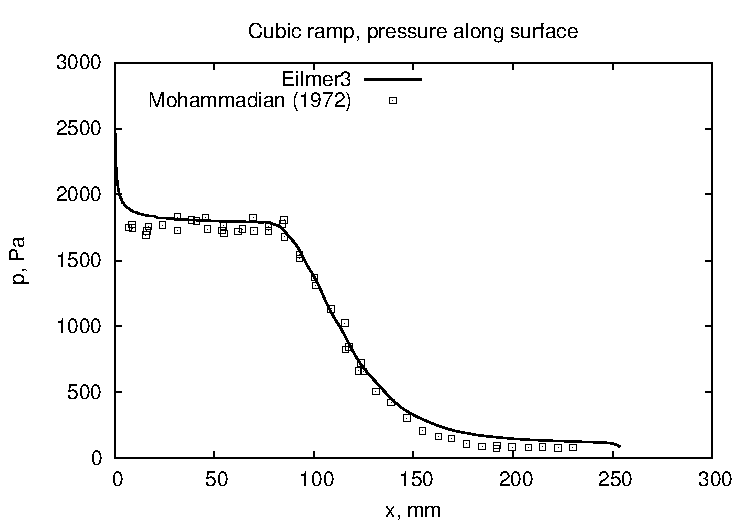
\includegraphics[width=0.5\textwidth]
    {../2D/convex-ramp/thermo-noneq/surface-pressure.pdf}\label{fig:convex-ramp-noneq-surface-pressure}}
 \subfloat[Heat transfer.]{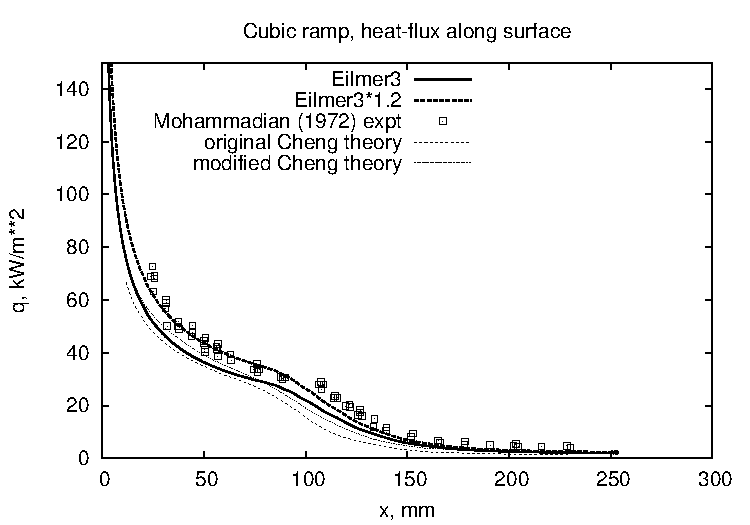
\includegraphics[width=0.5\textwidth]
    {../2D/convex-ramp/thermo-noneq/surface-heat-transfer.pdf}\label{fig:convex-ramp-noneq-heat-transfer}}
 \caption{Distribution of pressure and heat transfer along the concave ramp.
   Simulation data is recorded at $t$=1\,ms into the simulation.
   Experimental data is from Ref.\,\cite{mohammadian_1972a}.}
 \label{fig:convex-ramp-noneq-data-compare}
\end{figure}


\bigskip
\subsection{Postprocessing to get heat transfer}
\label{convex-ramp-noneq-post-processing}
%
The scripts below use the functions imported from \verb!e3_flow.py!
at a slightly higher level than in the cone20 example.
The first extracts the data for the cell nearest to the ramp surface
and uses that data to compute the expected shear stress and heat transfer at the surface.

\noindent
\topbar
\lstinputlisting[language={}]{../2D/convex-ramp/thermo-noneq/surface_properties.py}
\bottombar

\subsection{Notes}
\begin{itemize}
 \item Plotting was done with the following GNUPlot scripts.
 \lstinputlisting[language={}]{../2D/convex-ramp/thermo-noneq/surface-pressure.gnuplot}
 \lstinputlisting[language={}]{../2D/convex-ramp/thermo-noneq/surface-heat-transfer.gnuplot}
\end{itemize}
